\documentstyle[graphicx,aps,multicol]{revtex}
\draft

\begin{document}

\title{Level densities in $^{56,57}$Fe and $^{96,97}$Mo}
\author{A.~Schiller,$^{1}$\footnote{Electronic address: 
schiller@nscl.msu.edu}, E.~Tavukcu,$^{1,2,3,4}$ L.A.~Bernstein,$^1$ 
P.E.~Garrett,$^1$ M.~Guttormsen,$^5$ M.~Hjorth-Jensen,$^5$ C.W.~Johnson,$^6$ 
G.E.~Mitchell,$^{2,3}$ J.~Rekstad,$^5$ S.~Siem,$^5$ A.~Voinov,$^7$ 
W.~Younes$^1$}
\address{$^1$ Lawrence Livermore National Laboratory, L-414, 7000 East Avenue, 
Livermore, California 94551, USA}
\address{$^2$ North Carolina State University, Raleigh, North Carolina 27695, 
USA}
\address{$^3$ Triangle Universities Nuclear Laboratory, Durham, North Carolina 
27708, USA}
\address{$^4$ Department of Physics, Osmangazi University, Meselik, Eskisehir, 
26480 Turkey}
\address{$^5$ Department of Physics, University of Oslo, N-0316 Oslo, Norway}
\address{$^6$ San Diego State University, San Diego, California 92182, USA}
\address{$^7$ Frank Laboratory of Neutron Physics, Joint Institute of Nuclear 
Research, 141980 Dubna, Moscow region, Russia}

\maketitle

\begin{abstract}
Level densities up close to the neutron binding energy have been extracted from
primary $\gamma$ spectra for $^{56,57}$Fe and $^{96,97}$Mo nuclei using 
($^3$He,$\alpha\gamma$) and ($^3$He,$^3$He$^\prime\gamma$) reactions on 
$^{57}$Fe and $^{97}$Mo targets. It is shown that statistical spectroscopy 
provides a useful tool in this mass region. Apparent step structures in the 
level-density curves are tentatively explained by a schematic microscopic model
comprised of single-particle level spacings and seniority-conserving and 
seniority-non-conserving interactions.
\end{abstract}

\pacs{PACS number(s): 21.10.Ma, 25.55.Hp, 27.40.+z, 27.60.+j}

\begin{multicols}{2}

The group at the Oslo Cyclotron Laboratory (OCL) has recently developed a new 
method (the so-called Oslo method) to extract the level density and radiative 
strength function from primary $\gamma$ spectra \cite{SB00}. The method can be
characterized as a further development of the sequential extraction method 
\cite{BB70,BE73}. The Oslo method has been extensively tested in the rare-earth
mass region which has led to many fruitful applications 
\cite{SB01,MG01,VG01,SG02}. However, whether this approach could be extended to
much lighter nuclei or to nuclei near closed shells was an open question. The 
first extension of the Oslo method outside the rare-earth region was to 
$^{27,28}$Si \cite{GM02}. For these nuclei a direct comparison was possible 
between the average of the tabulated discrete levels and the level density 
determined via the Oslo method. The overall agreement for the level density 
obtained via these two methods was excellent. This surprising agreement in such
light nuclei encouraged us to test the method in intermediate nuclei. In such 
nuclei the level density is sufficiently low that a purely statistical analysis
may not be appropriate, but the level density is sufficiently high that direct
counting methods fail. We chose to test the method on $^{56,57}$Fe and 
$^{96,97}$Mo.

The $^{56}$Fe nucleus was especially chosen due to astrophysical interest in 
this isotope. Partition functions of nuclei in this mass region, i.e., the 
Laplace transforms of their level densities, determine both the relative 
nuclear abundances in the late-time pre-supernova star \cite{BB79} and the 
high-temperature weak rates \cite{FF82} which again govern the mass of the 
homologous core in core-collapse supernovae. The nucleus $^{96}$Mo is of 
special interest in the investigation of the $|N-Z|$ dependence of level 
densities, since the mass 96 isobars are the only ones in the nuclear chart 
where one can find three different stable nuclei with $|N-Z|$ varying by eight 
units from $^{96}$Zr to $^{96}$Ru. Also the $|N-Z|$ dependence of level 
densities can have significant astrophysical importance \cite{AG01}, since many
reactions take place on unstable isotopes and therefore most of their reaction 
cross sections must be estimated by Hauser-Feshbach type calculations 
\cite{HF52,AA99}.

The purpose of the present work is to investigate the validity of the Oslo 
method in an intermediate mass region, to report on experimental level 
densities of $^{56,57}$Fe and $^{96,97}$Mo nuclei and to provide a schematic 
explanation of the observed step structures in these curves.

The experiments were performed at the MC-35 cyclotron at the OCL using a 
$\sim 2$-nA beam of 45-MeV $^3$He particles. The self-supporting targets were 
isotopically enriched to 94.7\% and 94.2\% and had thicknesses of 3.4~mg/cm$^2$
and 2.1~mg/cm$^2$ for $^{57}$Fe and $^{97}$Mo, respectively. Each experiment 
ran for approximately five days, and about 200,000 relevant particle-$\gamma$ 
coincidences were recorded in each analyzed reaction channel. The charged 
ejectiles were identified and their energies were measured in a ring of eight 
collimated Si $\Delta E$-$E$ telescopes placed at 45$^\circ$ with respect to 
the beam direction. The thicknesses of the front and end detectors were 140 and
3000~$\mu$m, respectively and shielding against $\delta$ electrons was achieved
with a 19-$\mu$m-thick Al foil. The distance from the target was 5~cm, giving a
total solid angle coverage of 0.3\% of $4\pi$, and the energy resolution was 
$\sim$0.3~MeV over the entire spectrum. The $\gamma$-rays were detected in 28 
collimated 5"x5" NaI(Tl) detectors collectively called CACTUS \cite{GA90} 
surrounding the target and particle detectors. The total efficiency of CACTUS 
was $\sim$15\% of $4\pi$ and the resolution was $\sim$6\% of the deposited 
energy at 1.3~MeV\@. In addition, one 60\% Ge(HP) detector was used in the 
setup to monitor the selectivity and populated spin distribution of the 
reactions. Raw $\alpha$-particle data are shown in Fig.\ \ref{fig:moraw} for 
the case of the $^{97}$Mo($^3$He,$\alpha$)$^{96}$Mo reaction, where discrete
transfer peaks are observed up to $\sim$6~MeV in excitation energy indicating 
the opening of the neutron $g_{9/2}$ shell.

>From the known $Q$-value and the reaction kinematics, the ejectile energy can 
be transformed into initial excitation energy of the residual nuclei. Using the
particle-$\gamma$ coincidence technique, each $\gamma$ ray can be assigned to a
cascade depopulating a certain initial excitation energy in the residual 
nucleus. The data are therefore sorted into total $\gamma$-ray spectra 
originating from different initial excitation energy bins. Every spectrum is 
then unfolded using a Compton-subtraction method which preserves the 
fluctuations in the original spectra and does not introduce further, spurious 
fluctuations \cite{GT96}. From the unfolded spectra, a primary $\gamma$ matrix
is constructed using the subtraction method of Ref.\ \cite{GR87}. The basic 
assumption behind this method is that the $\gamma$-ray decay pattern from any 
excitation energy bin is independent of whether states in this bin are 
populated directly via the ($^3$He,$\alpha$) or ($^3$He,$^3$He$^\prime$) 
reactions or indirectly via $\gamma$ decay from higher excited levels following
the initial nuclear reaction. This assumption is trivially fulfilled if one 
populates the same levels with the same weights within any excitation energy 
bin, since the decay branchings are properties of the levels and do not depend 
on the population mechanisms. On the other hand, if one populates, e.g., vastly
different spin distributions within one excitation energy bin via the two 
different population mechanisms, the $\gamma$-decay patterns should be 
different as well. As an example of the data analysis discussed in this 
paragraph, the raw, unfolded and primary $\gamma$ spectra are shown for the 
$^{57}$Fe($^3$He,$\alpha\gamma$)$^{56}$Fe and 
$^{57}$Fe($^3$He,$^3$He$^\prime\gamma$)$^{57}$Fe reactions in Fig.\ 
\ref{fig:feraw}.

Finally, the primary $\gamma$ matrix is factorized using the generalized 
Brink-Axel hypothesis \cite{Br55,Ax62}. The original hypothesis states that the
giant dipole resonance (GDR) can be built on every excited state, and that the 
properties of the GDR do not depend on the temperature of the nuclear state on 
which it is built. This hypothesis can be generalized to include not only the 
GDR but any type of nuclear excitation and results in the assumption that 
primary $\gamma$ spectra originating from the excitation energy $E$ can be 
factorized into a $\gamma$-ray transmission coefficient 
${\mathcal{T}}(E_\gamma)$, which depends only on the $\gamma$-transition energy
$E_\gamma$, and into the level density $\rho(E-E_\gamma)$ at the final energy.
This simple picture is complicated by the experimental fact that the Brink-Axel
hypothesis is violated at sufficiently high temperatures ($\agt 1$--2~MeV). 
Especially the width of the GDR has been shown to depend on temperature 
\cite{RA00}. Models based on Fermi-liquid theory suggest a $T^2$ dependence for
this effect \cite{KM83,Si86}. Within the rather low excitation-energy range 
under study in the present work, however, the temperature dependence of the 
$\gamma$-ray transmission coefficient is not so well established 
experimentally. For the purpose of this work, we assume therefore that (i) 
temperature changes weakly within our experimentally accessible excitation 
energy range (roughly $T\propto\sqrt{E}$), and (ii) variations of the 
$\gamma$-ray transmission coefficient with temperature are small (roughly a 
second-order effect in $T$ according to \cite{KM83}). Within these assumptions 
we can expect to replace the actual temperature dependence in 
${\mathcal{T}}(E_\gamma,T)$ by a constant, average value $\langle T\rangle$ of 
the temperature and thus, recover the applicability of the generalized 
Brink-Axel hypothesis. The systematic error we introduce by this approximation
is largest for the low-energy part ($\alt 2$--3~MeV) of the $\gamma$-ray 
transmission coefficient where it can reach $\sim$20\%.

The factorization of the primary $\gamma$ matrix into ${\mathcal{T}}(E_\gamma)$
and $\rho(E-E_\gamma)$ is determined by a least-$\chi^2$ fit to the primary 
$\gamma$ matrix, using no \sl a priori \rm assumptions about the functional 
form of either the level density or the $\gamma$-ray transmission coefficient 
\cite{SB00}. In the present work, the error estimate of the first-generation 
matrix has been improved over \cite{SB00} thereby decreasing spurious 
fluctuations in the resulting level densities and $\gamma$-ray transmission 
coefficients. An example to illustrate the quality of the fit is shown in Fig.\
\ref{fig:fgmo}, where for the $^{97}$Mo($^3$He,$^3$He$^\prime\gamma$)$^{97}$Mo 
reaction we compare the experimental primary $\gamma$ spectra from two 
different initial excitation energies to the least $\chi^2$ fit. Unfortunately,
the mathematical structure of the relevant equations in the least $\chi^2$ fit 
does not allow us to find a unique solution for the level density and 
$\gamma$-ray transmission coefficient. However, it has been shown that all 
solutions with the same $\chi^2$ can be obtained by the transformation of one 
randomly chosen solution according to \cite{SB00}
\begin{eqnarray}
\tilde{\rho}(E-E_\gamma)&=&A\exp[\alpha(E-E_\gamma)]\rho(E-E_\gamma)\\
\tilde{\mathcal{T}}(E_\gamma)&=&B\exp(\alpha E_\gamma){\mathcal{T}}(E_\gamma).
\end{eqnarray}
The three free parameters $A$, $B$, and $\alpha$ have to be determined to give 
the physically most relevant solution to the least $\chi^2$ fit using 
independent experimental information. The most common way is to count the 
number of discrete levels at low excitation energies \cite{FS96} and to use the
average neutron resonance spacing at $B_n$ to find values for $A$ and $\alpha$.
The remaining parameter $B$ is then determined using the average total 
radiative width of neutron resonances \cite{VG01}. In the case of $^{56}$Fe, 
there are no data on neutron resonances and thus, the information about the 
level density around $B_n$ in $^{56}$Fe has to be obtained by different means. 
In order to do so, we calculate the level density at $B_n$ in $^{57}$Fe using a
backshifted Fermi-gas expression with the parameterization of von Egidy \sl et 
al.\ \rm \cite{ES88}, where we apply an additional overall re-normalization 
factor to match the level density determined from neutron resonance spacings. 
Then, we use the same level-density parameterization (including the same 
re-normalization factor but with parameters appropriate for $^{56}$Fe) to 
calculate the level density at $B_n$ in $^{56}$Fe. Using this data point 
instead of the unknown average neutron resonance spacing, we proceed in the 
same way as for the other three nuclei \cite{SB00,Ta02}. The estimated level 
density of $^{56}$Fe at $B_n$ obtained in this manner is in good agreement with
experimental data obtained from particle evaporation studies \cite{FT84}.

In Fig.\ \ref{fig:levdens} we show the extracted level densities in 
$^{56,57}$Fe and $^{96,97}$Mo from the present data. The quality of the results
strongly suggests that statistical methods can be applied in this intermediate 
mass region. This is farther supported by, e.g., studies of the total $\gamma$ 
cascade after keV-neutron capture where it has been shown that sufficient 
averaging over initial states allows the description of the resulting $\gamma$ 
spectrum within the statistical model \cite{IM88}. Since the experimental 
evidence strongly implies that the Oslo method can provide valid results in 
this intermediate mass region, we focus on the physics implications of the 
experimental level densities.

The most striking features in the level-density curves in Fig.\ 
\ref{fig:levdens} are the steps starting at 2.9~MeV in $^{56}$Fe and 1.8~MeV in
$^{57}$Fe. These steps are verified in the level-density curves obtained from 
the counting of discrete levels. However, there are fluctuations due to the 
binning procedure, and the energy at which the discrete level scheme becomes 
incomplete (due to missing levels) is not known. As a result, evidence for step
structures from discrete level schemes must be only provisional. The 
combination of these two independent data sets provides much stronger evidence.
There is also a less pronounced, but still statistically significant, step 
structure at 1.2~MeV in $^{97}$Mo. This structure cannot be observed from 
counting of discrete states -- it is too high in energy and the level density 
is too large.\footnote{It is worth noting that the counting of discrete levels 
provides an approximately complete level density up only to a level density 
value of about 60 levels per MeV in the four nuclei under study. This value can
be extended using high-resolution $\gamma$ detectors and the measurement of 
$\gamma$ excitation functions from neutron inelastic scattering. However, even
for the best investigated nucleus thus far -- $^{112}$Cd (see Ref.\cite{GL01}) 
this value has been extended only to 160 levels per MeV\@. Even this best case 
would not be sufficient to perform complete spectroscopy up to the particle 
separation energy for any of the four nuclei measured in the present 
experiment.} (A possible step structure in $^{96}$Mo at 2.0~MeV is probably too
smeared out in the present experimental data but might still be visible in the 
discrete level scheme.) It has been established in the rare-earth region that 
such low-lying step structures are connected to the breaking of the first 
nucleon Cooper pair \cite{MB99}. It is therefore reasonable to assume that the 
same is true for the lighter mass regions. The additional step at 6~MeV in the 
level-density curve of $^{96}$Mo may be due to the opening of the $g_{9/2}$ 
shell which should occur at this excitation energy (see Fig.\ \ref{fig:moraw}).
A future systematic investigation of the Mo nuclei may shed more light on this 
issue. The structures in the level density data of the Fe nuclei at high 
excitation energies presumably reflect fluctuations due to poorer statistics.

The difference in binding energy between the even and odd systems is a measure 
for pairing correlation and can be calculated from the three-mass indicator of 
Dobaczewski \sl et al.\ \rm \cite{DM01}. This indicator yields 1.3~MeV and 
1.1~MeV for the Fe and Mo nuclei, respectively, which agrees well with the
differences in excitation energy for the first steps in the level-density 
curves. Thus, the steps in neighboring nuclei appear at the same 'effective' 
excitation energy, i.e., the excitation energy corrected for the contribution 
to the binding energy due to neutron-pairing correlations. Further, the proton 
pairing energies are 0.7~MeV and 1.0~MeV for the $^{57}$Fe and $^{97}$Mo 
nuclei, respectively. These energies should now correspond to the excitation 
energies of the steps in the two odd nuclei. However, the steps are delayed in 
excitation energy by 1.1~MeV and 0.2~MeV for these two nuclei. This might be 
explained by the fact that one not only has to invest the energy to break a 
proton Cooper pair but also at least one of the unpaired protons has to be 
promoted to the next unoccupied single-particle level. The average spacing of 
those levels can also be calculated using the Dobaczewski three-mass indicator,
giving 1.9~MeV and 1.3~MeV in the two cases. Clearly the higher single-particle
spacing for $^{56}$Fe as compared to $^{97}$Mo leads to a larger delay in 
excitation energy for the appearance of the step structure. However, the exact 
excitation energy cannot be estimated from binding energies, since it will 
depend on the exact location of the Fermi energy within the single-particle 
level scheme.

Another complication might arise from the effect of seniority non-conserving
interactions, which mix configurations of different seniority and smooth out 
the step structures in the level densities.\footnote{The effect of pairing 
correlations on the nuclear level density (mostly utilizing the concept of a 
nuclear temperature) has been investigated by numerous authors in the past, the
first being Sano and Yamasaki \cite{SY63}. In this work, however, we chose an 
entirely microscopic approach.} To investigate this, we have performed a model 
calculation. In the model we assume a system of eight particles scattered into 
an equidistant single-particle level scheme with eight doubly-degenerate 
levels. As residual interactions we consider a pairing interaction and a 
seniority non-conserving interaction. Thus, the model Hamiltonian is written as
\begin{eqnarray}
\lefteqn{\widehat{H}=\epsilon\sum_{i=1}^8ia_i^\dagger a_i-\frac{1}{2}G
\sum_{i,j=1}^8a_i^\dagger a_{\bar{\imath}}^\dagger a_{\bar{\jmath}}a_j}
\nonumber\\
&&-\frac{1}{2}\kappa\sum_{i,j,k,l=1}^8W_{ijkl}a_i^\dagger a_j^\dagger 
a_ka_l,
\label{eq:ham}
\end{eqnarray}
where $a^\dagger$ and $a$ are Fermion creation and annihilation operators and 
the labels with bars stand for time reversed orbits. The single-particle level
spacing $\epsilon$, the strength $G$ of the pairing interaction and the 
strength $\kappa$ of the seniority non-conserving interaction $W$ are the only 
macroscopic parameters of the model. This model with good seniority, i.e., the 
case of $\kappa=0$, has already been diagonalized in Ref.\ \cite{GB00}, and the
dotted line in Fig.\ \ref{fig:calc} gives the distribution of eigenvalues with 
excitation energy, i.e., the exact level density of the model. The individual 
bumps contain mainly levels with the same seniority, thus the step structures 
in the level density can be explained by the consecutive breaking of nucleon 
Cooper pairs. However, the experimental data show that in general the steps are
much smoother than in such a simple model calculation indicating the need for 
seniority non-conserving terms in the Hamiltonian.

An important contribution to seniority breaking comes from quadrupole 
collectivity, which can change rapidly with mass number for the nuclei under 
study. Strong, residual quadrupole-quadrupole interactions can lead to 
deformation of the nucleus and to a modification of the single-particle level 
spacing. Unfortunately, our simple model cannot incorporate a realistic 
quadrupole-quadrupole interaction; the smoothing of the level density, however,
should not depend too much on the details of the seniority non-conserving 
residual interaction. We choose therefore to model the quadrupole-quadrupole 
interaction by a random two-body interaction \cite{MF75} of roughly equivalent 
strength where all the pairing-like terms have been set to zero i.e., the 
$W_{ijkl}$ in Eq.\ (\ref{eq:ham}) are Gaussian random numbers of mean zero and 
width equal to one, except for the cases of $j=\bar{\imath}$ and $k=\bar{l}$ 
where $W_{i\bar{\imath}\bar{l}l}=0$.

Since in this more general case Eq.\ (\ref{eq:ham}) does not have good 
seniority, exact diagonalization of the model Hamiltonian has to be performed 
within the full model space which is computationally very demanding, as one 
requires \it all \rm levels, not just the lowest. For eight particles in eight 
doubly-degenerate states there are 12870 states (counting all magnetic 
substates). The number of levels (not counting magnetic substates) equals the 
number of states with spin projection $J_z=0$, thus yielding 4900 levels. For 
the present calculations, we used $\epsilon=0.25$~MeV, $G=0.5$~MeV, and 
$\kappa\approx 0$~MeV (pure pairing) and $\kappa=0.14$~MeV (pairing+random 
interaction). In Fig.\ \ref{fig:calc}, we show the resulting level densities of
the two calculations. The resolved bumps with definite seniority in the pure 
pairing case are smeared out by the random interaction. The gaps between the 
bumps are rapidly being filled, while the bumps themselves are degraded into a 
step structure quite similar to the step structure seen in the experimental 
level-density curves of the iron nuclei. The occurrence of the step structure 
in the calculation is actually quite sensitive to the exact choice of the 
strength of the random interaction. A weak random interaction 
($\kappa\le 0.1$~MeV) does not fill the gaps between the bumps, a much stronger
random interaction ($\kappa\ge 0.2$~MeV) produces a more smeared-out step 
structure in the level-density curve similar to the Mo data, indicating the 
presence of relatively stronger seniority non-conserving interactions in the Mo
nuclei. The range of values that produces good qualitative agreement with the 
Fe data is about 0.13~MeV$\le\kappa\le 0.16$~MeV\@. However, due to the 
simplicity of the model, no attempt has been made to achieve quantitative 
agreement between the model and the experimental data.

In conclusion, we have shown that statistical methods like the Oslo method can
be applied to an intermediate mass region where the level density is still 
relatively low. New experimental data on level densities below $B_n$ in 
$^{56,57}$Fe and $^{96,97}$Mo have been presented. Step structures in the 
level-density curves have been tentatively related to the breaking of nucleon 
Cooper pairs. The position of the step structures in energy depends on the 
exact location of the Fermi energy in the single-particle level scheme. The 
smoothness of the step structures depends on the strength of the seniority 
non-conserving interactions, e.g., the quadrupole-quadrupole interaction 
relative to the pairing interaction and the average single-particle level 
spacing. The more pronounced step structures in the level density data of Fe 
compared to Mo indicate relatively stronger seniority non-conserving 
interactions in the latter case. Our schematic calculations where random 
two-body interactions were used to model residual seniority non-conserving 
interactions show that the low-energy part of theoretical level-density curves 
are very sensitive to the relative strengths of the different terms in the 
model Hamiltonian. The present experimental data therefore suggest a new 
approach for possible theoretical investigations of the pairing and 
quadrupole-quadrupole interactions.

Part of this work was performed under the auspices of the U.S. Department of 
Energy by the University of California, Lawrence Livermore National Laboratory 
under Contract No.\ W-7405-ENG-48. Financial support from the Norwegian 
Research Council (NFR) is gratefully acknowledged. G.M. acknowledges support by
a U.S. Department of Energy grant with No.\ DE-FG02-97-ER41042. One of the 
authors (A.S.) would like to thank Jason Pruet for interesting discussions.

\begin{references}
\bibitem{SB00}A. Schiller, L. Bergholt, M. Guttormsen, E. Melby, J. Rekstad, 
and S. Siem, Nucl.\ Instrum.\ Methods Phys.\ Res.\ A \bf 447\rm, 498 (2000).
\bibitem{BB70}G. A. Bartholomew, I. Bergqvist, E. D. Earle, and A. J. Ferguson,
Can.\ J. Phys.\ \bf 48\rm, 687 (1970).
\bibitem{BE73}G. A. Bartholomew, E. D. Earle, A. J. Ferguson, J. W. Knowles, 
and M. A. Lone, Adv.\ Nucl.\ Phys.\ \bf 7\rm, 229 (1973). 
\bibitem{SB01}A. Schiller, A. Bjerve, M. Guttormsen, M. Hjorth-Jensen, F. 
Ingebretsen, E. Melby, S. Messelt, J. Rekstad, S. Siem, and S. W. 
{\O}deg{\aa}rd, Phys.\ Rev.\ C \bf 63\rm, 021306(R) (2001).
\bibitem{MG01}E. Melby, M. Guttormsen, J. Rekstad, A. Schiller, S. Siem, and A.
Voinov, Phys.\ Rev.\ C \bf 63\rm, 044309 (2001).
\bibitem{VG01}A. Voinov, M. Guttormsen, E. Melby, J. Rekstad, A. Schiller, and
S. Siem, Phys.\ Rev.\ C \bf 63\rm, 044313 (2001).
\bibitem{SG02}S. Siem, M. Guttormsen, K. Ingeberg, E. Melby, J. Rekstad, A.
Schiller, and A. Voinov, Phys.\ Rev.\ C \bf 65\rm, 044318 (2002).
\bibitem{GM02}M. Guttormsen, E. Melby, J. Rekstad, S. Siem, A. Schiller, T. 
L{\"o}nnroth, and A. Voinov, J. Phys.\ G \bf 29\rm, 263 (2003).
\bibitem{BB79}H.A. Bethe, G.E. Brown, J. Applegate, and J.M. Lattimer, Nucl.\ 
Phys.\ \bf A324\rm, 487 (1979).
\bibitem{FF82}G.M. Fuller, W.A. Fowler, and M.J. Newman, Ap.\ J. \bf 252\rm, 
715 (1982).
\bibitem{AG01}S. I. Al-Quraishi, S. M. Grimes, T. N. Massey, and D. A. Resler,
Phys.\ Rev.\ C \bf 63\rm, 065803 (2001).
\bibitem{HF52}W. Hauser and H. Feshbach, Phys.\ Rev.\ \bf 87\rm, 366 (1952).
\bibitem{AA99}C. Angulo, \sl et al.\rm, Nucl.\ Phys.\ \bf A656\rm, 3 (1999).
\bibitem{GA90}M. Guttormsen, A. Atac, G. L{\o}vh{\o}iden, S. Messelt, T. 
Rams{\o}y, J. Rekstad, T. F. Thorsteinsen, T. S. Tveter, and Z. Zelazny, Phys.\
Scr.\ \bf T32\rm, 54 (1990). 
\bibitem{CM73}S. Cochavi, A. Moalem, D. Ashery, J. Alster, G. Bruge, and A. 
Chaumeaux, Nucl.\ Phys.\ \bf A211\rm, 21 (1973).
\bibitem{GT96}M. Guttormsen, T. S. Tveter, L. Bergholt, F. Ingebretsen, and J.
Rekstad, Nucl.\ Instrum.\ Methods Phys.\ Res.\ A \bf 374\rm, 371 (1996).
\bibitem{GR87}M. Guttormsen, T. Rams{\o}y, and J. Rekstad, Nucl.\ Instrum.\ 
Methods Phys.\ Res.\ A \bf 255\rm, 518 (1987).
\bibitem{Br55}D. M. Brink, Ph.D. thesis, Oxford University, 1955.
\bibitem{Ax62}P. Axel, Phys.\ Rev.\ \bf 126\rm, 671 (1962).
\bibitem{RA00}E. Ramakrishnan, \sl et al.\rm, Phys.\ Lett.\ B \bf 383\rm, 252 
(2000). 
\bibitem{KM83}S.G. Kadmenski\u\i, V.P. Markushev, and V.I. Furman, Yad.\ Fiz.\ 
\bf 37\rm, 277 (1983), [Sov.\ J. Nucl.\ Phys.\ \bf 37\rm, 165 (1983)]. 
\bibitem{Si86}V.K. Sirotkin, Yad.\ Fiz.\ \bf 43\rm, 570 (1986), [Sov.\ J. 
Nucl.\ Phys.\ \bf 43\rm, 362 (1986)].
\bibitem{FS96}R.B. Firestone and V.S. Shirley, \sl Table of Isotopes\rm, 8th 
ed.\ (Wiley, New York, 1996), Vol.\ II.
\bibitem{ES88}T. von Egidy, H. H. Schmidt, and A. N. Bekhami, Nucl.\ Phys.\ \bf
A481\rm, 189 (1988).
\bibitem{Ta02}E.Tavukcu, Ph.D. thesis, North Carolina State University, 2002.
\bibitem{FT84}R. Fischer, G. Traxler, M. Uhl, and H. Vonach, Phys.\ Rev.\ C \bf
30\rm, 72 (1984).
\bibitem{IM88}Masayuki Igashira, Hiroshi Matsumoto, Toshio Uchiya\-ma, and 
Hideo Kitazawa, in \sl Proceedings of the International Conference on Nuclear 
Data for Science and Technology\rm, Mito, Japan, 1988, edited by S. Igarasi 
(Saikon Publishing Co. Ltd., Tokyo, 1988), p.\ 67.
\bibitem{GL01}P.E. Garrett, H. Lehmann, J. Jolie, C.A. McGrath, Minfang Yeh, W.
Younes, and S.W. Yates, Phys.\ Rev.\ C \bf 64\rm, 024316 (2001).
\bibitem{MB99}E. Melby, L. Bergholt, M. Guttormsen, M. Hjorth-Jensen, F. 
Ingebretsen, S. Messelt, J. Rekstad, A. Schiller, S. Siem, and S. W. 
{\O}deg{\aa}rd, Phys.\ Rev.\ Lett.\ \bf 83\rm, 3150 (1999).
\bibitem{DM01}J. Dobaczewski, P. Magierski, W. Nazarewicz, W. Satu{\l}a, and Z.
Szyma{\'n}ski, Phys.\ Rev.\ C \bf 63\rm, 024308 (2001).
\bibitem{SY63}Mitsuo Sano and Shuichiro Yamasaki, Prog.\ Theo.\ Phys.\ bf 
29\rm, 397 (1963).
\bibitem{GB00}M. Guttormsen, A. Bjerve, M. Hjorth-Jensen, E. Melby, J. Rekstad,
A. Schiller, S. Siem, and A. Beli{\'c}, Phys.\ Rev.\ C \bf 62\rm, 024306 
(2000).
\bibitem{MF75}K.K. Mon and J.B. French, Ann.\ Phys.\ (N.Y.) \bf 95\rm, 90 
(1975).




\end{references}

\end{multicols}

\clearpage

\begin{figure}\centering
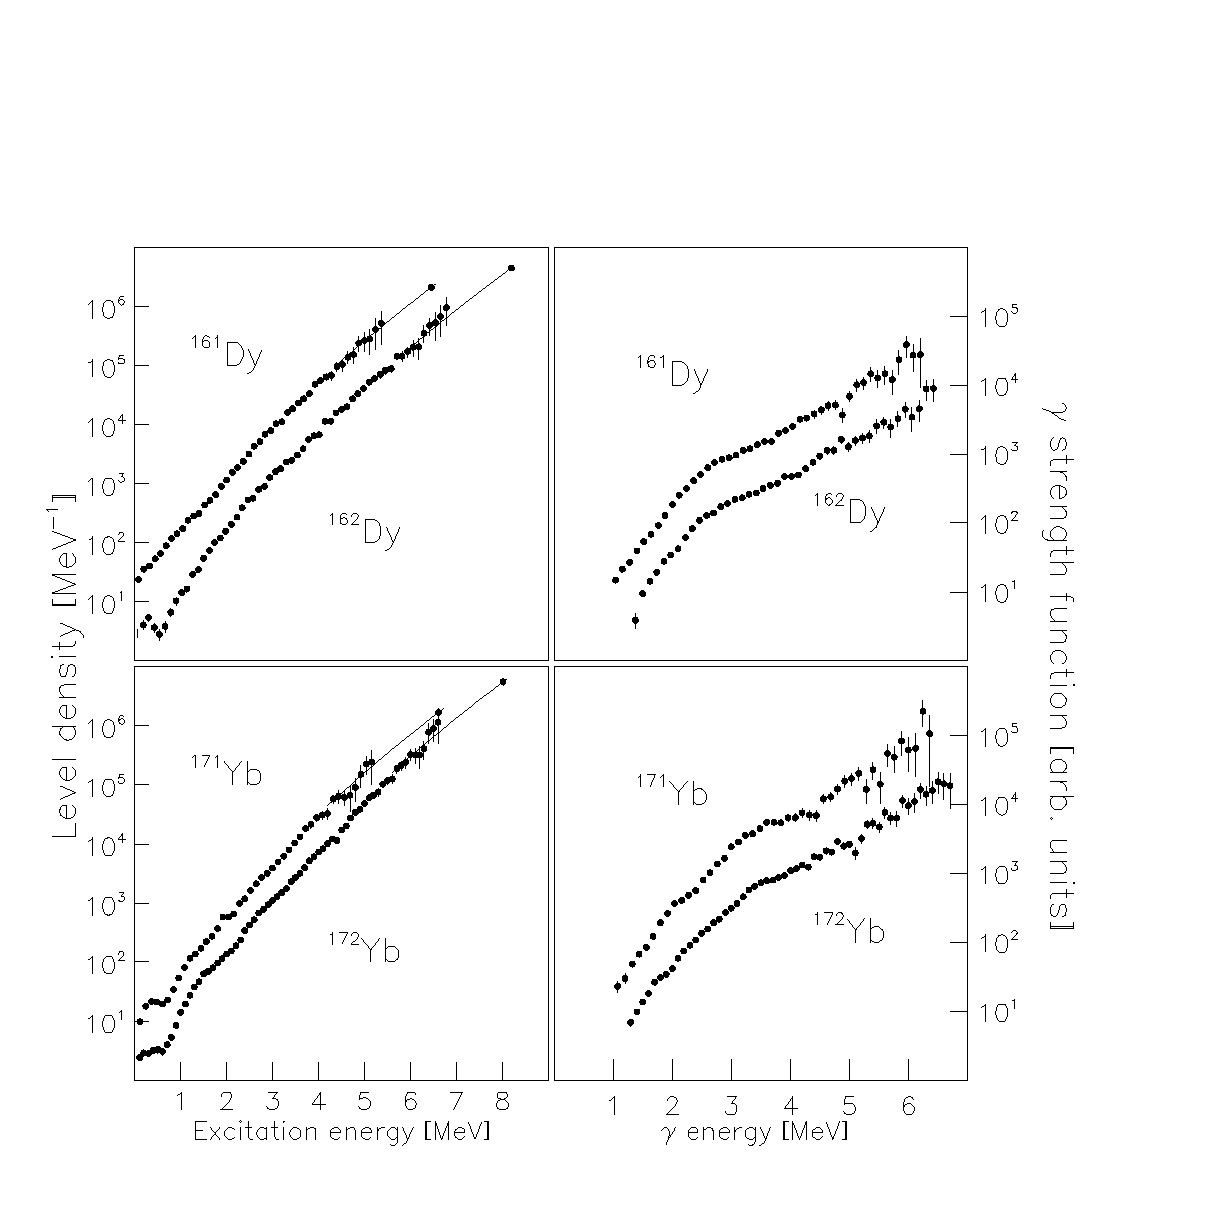
\includegraphics[totalheight=17.9cm]{fig1.eps}
\caption{Singles $\alpha$ spectrum (upper panel) and $\alpha$-$\gamma$ 
coincidence spectrum (lower panel) for the $^{97}$Mo($^3$He,$\alpha$)$^{96}$Mo 
reaction. At the neutron binding energy $B_n$, the coincidence spectrum shows a
rapid decrease reflecting the lower $\gamma$ multiplicity in the decay from 
low-lying states in $^{95}$Mo which are populated by neutron emission. The 
transfer peaks to the first three states are well known from the $(p,d)$ 
reaction \protect\cite{CM73}. The strong transfer peak at 5.3~MeV has not been 
observed previously, and presumably indicates the opening of the $g_{9/2}$ 
shell at this energy.}
\label{fig:moraw}
\end{figure}

\clearpage

\begin{figure}\centering
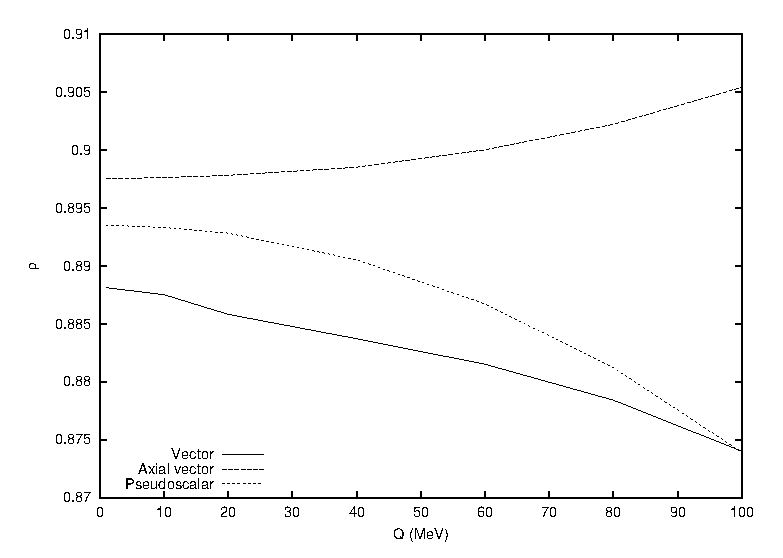
\includegraphics[totalheight=11.9cm]{fig2.eps}
\caption{Raw, unfolded, and primary $\gamma$ spectra from the 
$^{57}$Fe($^3$He,$\alpha\gamma$)$^{56}$Fe reaction at 5~MeV excitation energy 
(upper panels) and from the $^{57}$Fe($^3$He,$^3$He$^\prime\gamma$)$^{57}$Fe 
reaction at 6.2-MeV excitation energy (lower panels).}
\label{fig:feraw}
\end{figure}

\clearpage

\begin{figure}\centering
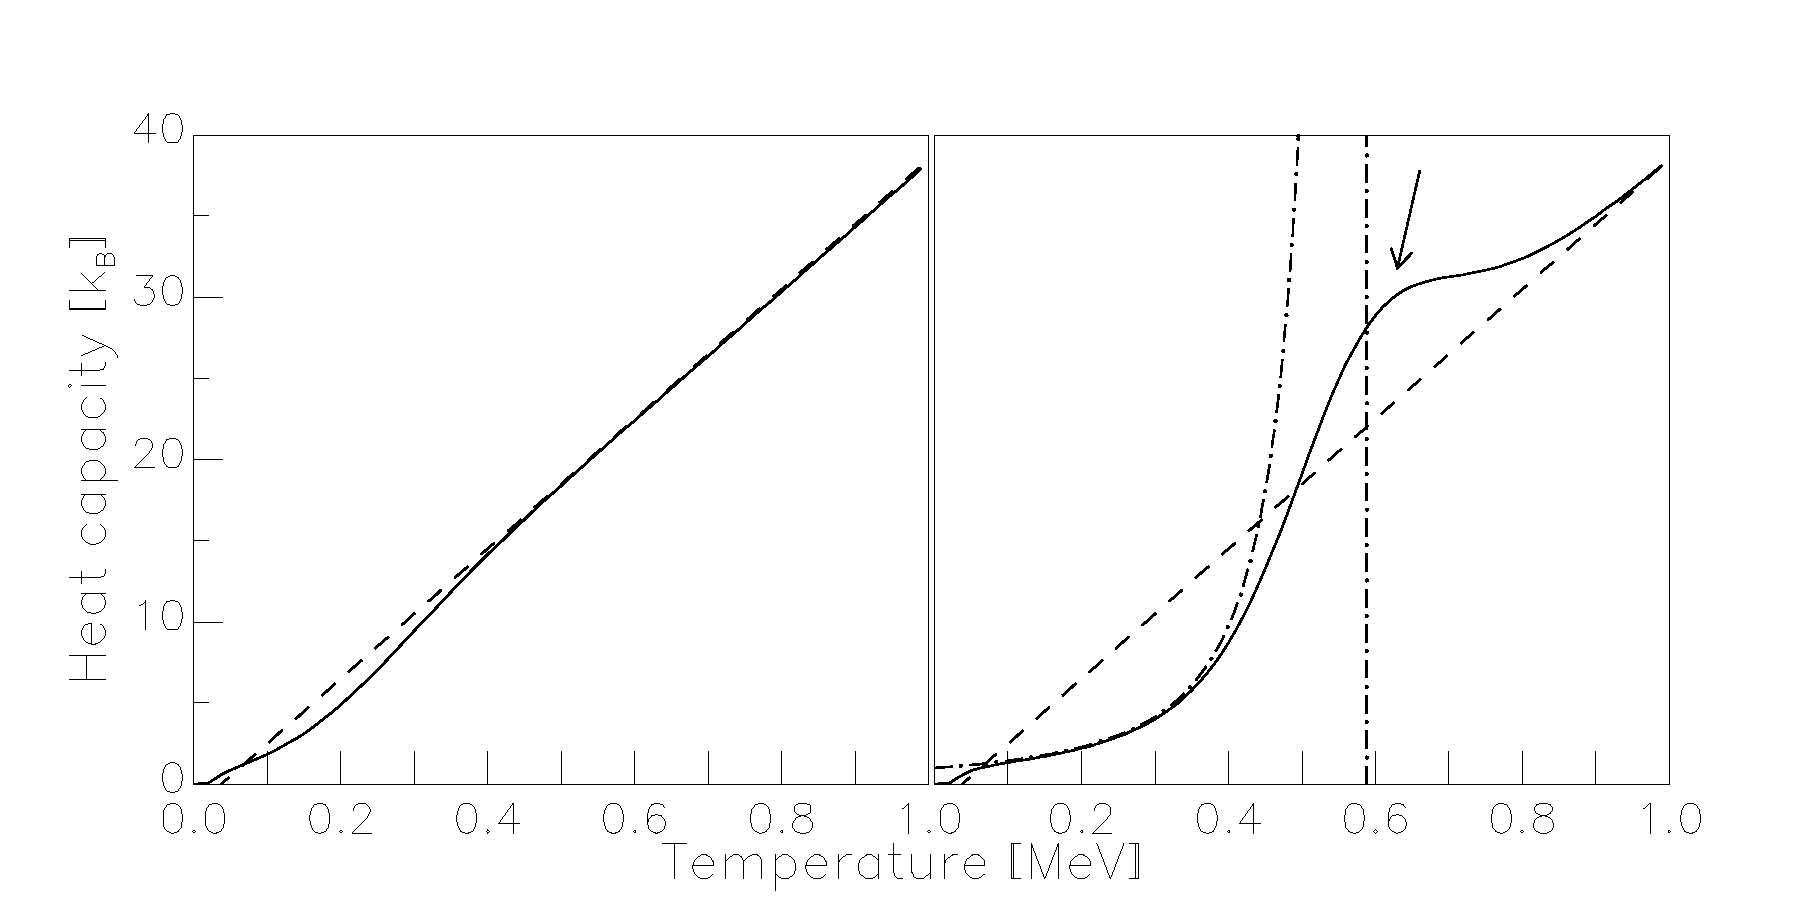
\includegraphics[totalheight=8.9cm]{fig3.eps}
\caption{Experimental primary $\gamma$ spectra (data points with error bars) at
two different initial excitation energies (indicated in the figure) compared to
the least $\chi^2$ fit (solid lines) for the 
$^{97}$Mo($^3$He,$^3$He$^\prime\gamma$)$^{97}$Mo reaction. The fit is performed
simultaneously to the entire primary $\gamma$ matrix of which the two displayed
spectra are only a small fraction. The first generation spectra are normalized
to one at each excitation energy bin.}
\label{fig:fgmo}
\end{figure}

\clearpage

\begin{figure}\centering
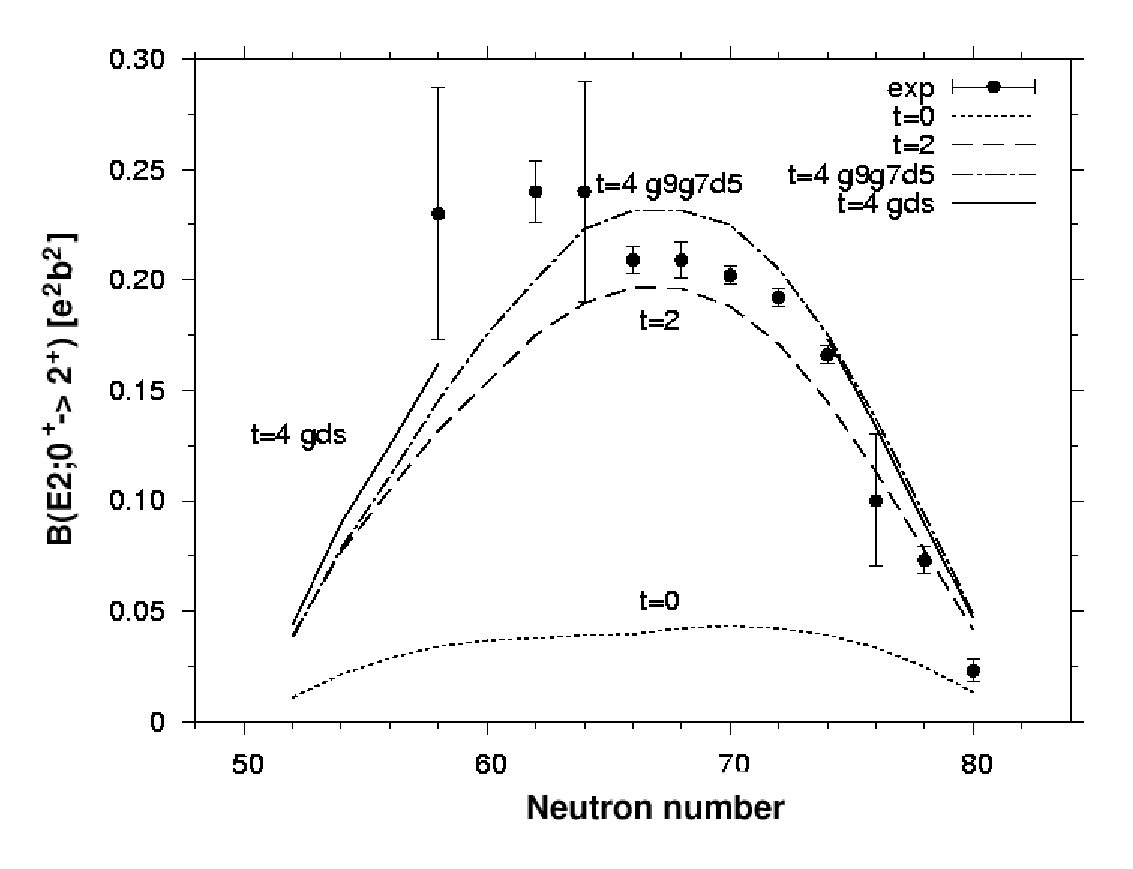
\includegraphics[totalheight=8.9cm]{fig4.eps}
\caption{Experimental level densities for the four nuclei under study (full and
open symbols represent even and odd nuclei, respectively). Wherever available, 
level density data from neutron resonance spacings have been added (triangles).
The square represents level density data from a particle evaporation study 
\protect\cite{FT84}. The smooth solid curves are the re-normalized level 
density parameterizations according to von Egidy \sl et al.\ \rm 
\protect\cite{ES88}. The jagged solid lines are level density information from
counting of discrete levels as given in the Table of Isotopes 
\protect\cite{FS96}. Apparent step structures in the level densities are marked
by arrows. In the level density of $^{56}$Fe, the bump and the plateau at 
0.8~MeV and 2.0~MeV, respectively, are due to the first and second excited 
states.}
\label{fig:levdens}
\end{figure}

\clearpage

\begin{figure}\centering
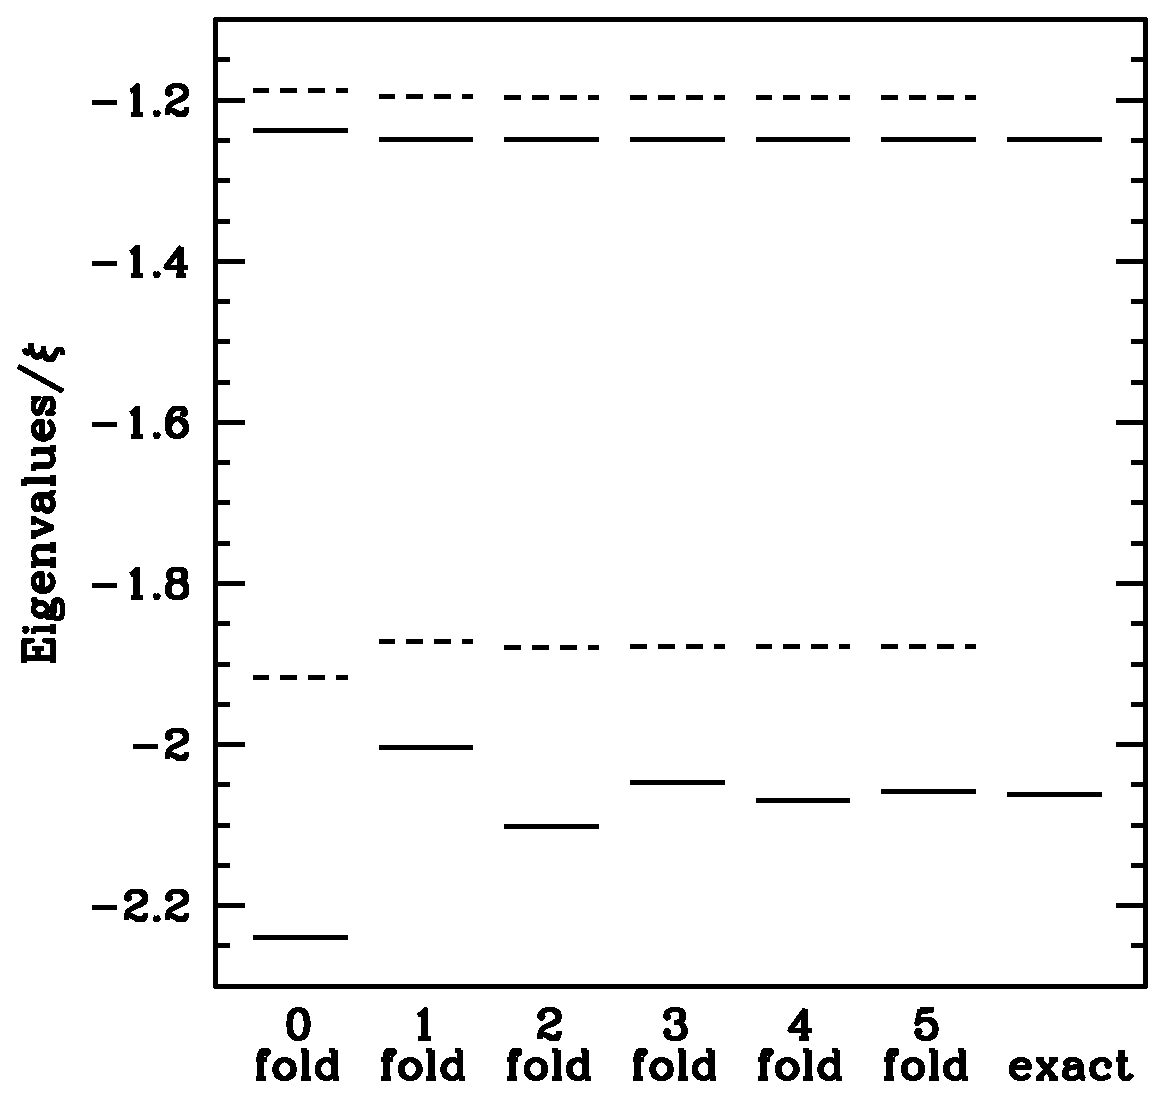
\includegraphics[totalheight=8.9cm]{fig5.eps}
\caption{Level density as function of excitation energy. Model calculation 
(dotted line) using the Hamiltonian of Eq.\ (\protect\ref{eq:ham}) with 
$\epsilon=0.25$~MeV, $G=0.5$~MeV, and $\kappa\approx 0$~MeV\@. Adding a random 
two-body interaction with the strength $\kappa=0.14$~MeV (solid line) results 
in a step structure similar to what is seen in the experimental level-density 
curve of the iron nuclei.}
\label{fig:calc}
\end{figure}

\end{document}
